\documentclass{beamer}

\usepackage[francais]{babel}
\usepackage[utf8]{inputenc}
\usepackage[T1]{fontenc}
\usepackage{lmodern}
\usepackage{tikz}

\usepackage{color}
\definecolor{UPMCEngagementBlueA}   {RGB}{140,184,198}
\definecolor{UPMCEngagementBlueB}   {RGB}{92,127,146}
\definecolor{UPMCEngagementBlueC}   {RGB}{75,146,219}
\definecolor{UPMCEngagementBlueD}   {RGB}{33,49,77}
\definecolor{UPMCEngagementYellowA} {RGB}{254,209,0}
\definecolor{UPMCEngagementYellowB} {RGB}{198,172,0}
\definecolor{UPMCEngagementGreen}   {RGB}{64,74,41}
\definecolor{UPMCCorporateGreen}    {RGB}{182,191,0}
\definecolor{UPMCExcellenceOrangeA} {RGB}{224,82,6}
\definecolor{UPMCExcellenceOrangeB} {RGB}{225,160,47}
\definecolor{UPMCCorporateMarron}   {RGB}{145,120,91}
\definecolor{UPMCInnovationCoolGray}{RGB}{97,99,101}

\colorlet{BgTransition}{UPMCInnovationCoolGray}

\usetheme{Madrid}

\usecolortheme{themeperso1}
\usecolortheme{themeperso2}
\setbeamertemplate{itemize items}[default]
\setbeamertemplate{enumerate items}[default]

\AtBeginSection[] % pour ne pas afficher le sommaire \section*
{
  \begin{frame}<beamer>
    \frametitle{Outline}
    \tableofcontents[currentsection]
  \end{frame}
}

\AtBeginSubsection[] % pour ne pas afficher le sommaire \subsection*
{
  \begin{frame}<beamer>
    \frametitle{Outline}
    \tableofcontents[currentsection,currentsubsection]
  \end{frame}
}

\graphicspath{{images/}}


\begin{document}
%% ---------------------------------------------------------------------------- 
%% ---------------------------------------------------------------------------- 
%% DEBUT SLIDES SUPPORT
%% ---------------------------------------------------------------------------- 
%% ---------------------------------------------------------------------------- 
\title{Worst case end-to-end response times of flows scheduled with FP/FIFO}

\author[]{CARVER Damien, BAUDRY Raphaël, DELPECH Clément, BOUTROS Darren, 
HADJARAB Naima}
\date{\today}
\frame{\titlepage} 

\section{Présentation du projet}
\begin{frame}{Enjeux}

\end{frame}


\section{Algorithme}
\begin{frame}{blabla}
 
\end{frame}


\section{Implémentation}
\begin{frame}{Première implémentation}

\end{frame}

\begin{frame}{Diagramme de Classes}
  \begin{figure}
    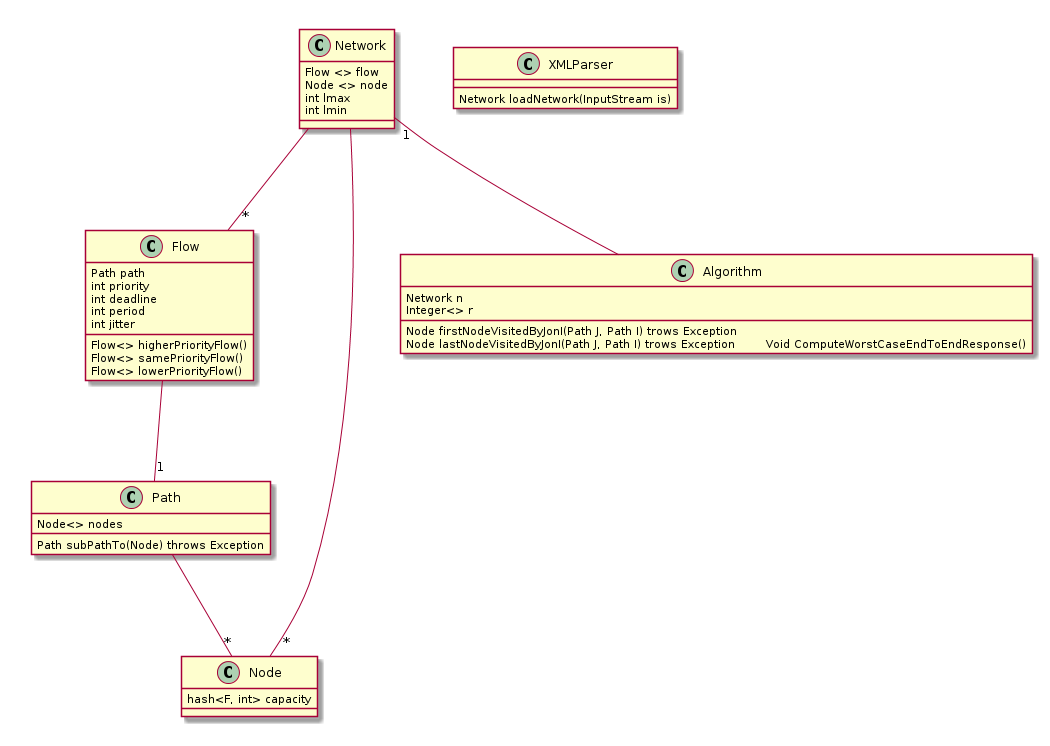
\includegraphics[scale=0.3]{../Rendu3/ClassDiagram.png}
  \end{figure}
\end{frame}

\begin{frame}{Résultats}

\end{frame}


\section{Tests}
\begin{frame}{}

\end{frame}


\section{Conclusion}
\begin{frame}{}

\end{frame}


\end{document}
